\documentclass{exam}
\usepackage[utf8]{inputenc}
\usepackage{lmodern}
\usepackage{microtype}

% \usepackage[parfill]{parskip}
\usepackage[dvipsnames]{xcolor}
\usepackage{amsmath}
\usepackage{amsfonts}
\usepackage{amsthm}
\usepackage{siunitx}
\DeclareSIUnit\year{yr}
\DeclareSIUnit\foot{ft}
\DeclareSIUnit\litre{\liter}

\usepackage{skull}

\usepackage{pgfplots}
\usepgfplotslibrary{polar}
\pgfplotsset{compat=1.11}
\usepgfplotslibrary{statistics}
\usepackage{graphicx}
\usepackage{sidecap}
\sidecaptionvpos{figure}{c}
\usepackage{float}
\usepackage{gensymb}
\usepackage{tkz-euclide}
\usetkzobj{all}
\usepackage{commath}
\usepackage{hyperref}
\usepackage{enumitem}
\usepackage{wasysym}
\usepackage{multicol}
\usepackage{mathtools}
\usepackage{tcolorbox}
\usepackage{tabularx}
\usepackage[version=4]{mhchem}
\usepackage{changepage}
\usepackage{listings}
\lstset{basicstyle=\ttfamily\linespread{0.8}\small}

\renewcommand*{\thefootnote}{\fnsymbol{footnote}}

\newtheorem*{thm}{Theorem}
\newtheorem*{iden}{Identity}
\newtheorem*{lemma}{Lemma}
\newtheorem{obs}{Observation}
\theoremstyle{definition}
\newtheorem*{defn}{Definition}
\newtheorem*{ex}{Example}
\newtheorem{con}{Construction}
\newtheorem*{alg}{Algorithm}

\newtheoremstyle{break}
  {\topsep}{\topsep}%
  {\itshape}{}%
  {\bfseries}{}%
  {\newline}{}%
\theoremstyle{break}
\newtheorem*{bthm}{Theorem}

% russian integral
\usepackage{scalerel}
\DeclareMathOperator*{\rint}{\scalerel*{\rotatebox{17}{$\!\int\!$}}{\int}}

% \DeclareMathOperator*{\rint}{\int}

\pgfplotsset{vasymptote/.style={
    before end axis/.append code={
        \draw[densely dashed] ({rel axis cs:0,0} -| {axis cs:#1,0})
        -- ({rel axis cs:0,1} -| {axis cs:#1,0});
    }
}}

% \pointsinrightmargin
\boxedpoints
\pointname{}

\newcommand{\questioA}{\question[\texttt{\textbf{\color{Cerulean} A}}]}
\newcommand{\questioM}{\question[\texttt{\textbf{\color{PineGreen} M}}]}
\newcommand{\questioE}{\question[\texttt{\textbf{\color{WildStrawberry} E}}]}
\newcommand{\questioS}{\question[\texttt{\textbf{\color{Goldenrod} S}}]}
\newcommand{\questioO}{\question[\texttt{\textbf{\color{BurntOrange} O}}]}

\newcommand{\parA}{\part[\texttt{\textbf{\color{Cerulean} A}}]}
\newcommand{\parM}{\part[\texttt{\textbf{\color{PineGreen} M}}]}
\newcommand{\parE}{\part[\texttt{\textbf{\color{WildStrawberry} E}}]}
\newcommand{\parS}{\part[\texttt{\textbf{\color{Goldenrod} S}}]}
\newcommand{\parO}{\part[\texttt{\textbf{\color{BurntOrange} O}}]}

\newcommand{\subparA}{\subpart[\texttt{\textbf{\color{Cerulean} A}}]}
\newcommand{\subparM}{\subpart[\texttt{\textbf{\color{PineGreen} M}}]}
\newcommand{\subparE}{\subpart[\texttt{\textbf{\color{WildStrawberry} E}}]}
\newcommand{\subparS}{\subpart[\texttt{\textbf{\color{Goldenrod} S}}]}
\newcommand{\subparO}{\subpart[\texttt{\textbf{\color{BurntOrange} O}}]}

\newcommand{\mainHeader}[2]{\section*{NCEA Level 2 Mathematics\\#1. #2}}
\newcommand{\mainHeaderHw}[2]{\section*{NCEA Level 2 Mathematics (Homework)\\#1. #2}}
\newcommand{\seealso}[1]{\begin{center}\emph{See also #1.}\end{center}}
\newcommand{\drills}[1]{\begin{center}\emph{Drill problems: #1.}\end{center}}
\newcommand{\basedon}[1]{\begin{center}\emph{Notes largely based on #1.}\end{center}}

\begin{document}

\section*{NCEA Level 2 Mathematics\\Year 11 diagnostics}
These questions are at the level required for NCEA Level 1 mathematics. At a bare minimum, students starting Y12 should be comfortable
with those questions in part A. Students aiming for a merit or excellence in Level 2 should also revise the questions in part B.

\subsection*{Part A}
A calculator isn't needed.
\begin{questions}
  \question Write $ \frac{3}{4} - \frac{1}{3} $ as a single fraction.
  \question If $ a = 5 $ and $ b = a - 3 $, what is the value of $ 3a - b $?
  \question What possible values of $ x $ make the equation $ 3x - 8 = -4x + 34 $ true?
  \question What possible values of $ y $ make the equation $ x^2 - x = 20 $ true?
  \question Write $ \dfrac{x + 1}{x - 1} + \dfrac{x + 1}{x - 2} $ as a single fraction.
  \question Give the equation of the line through the two points $ (0,1) $ and $ (2,3) $.
  \question The two shorter sides of a right-angled triangle measure \SI{2}{\metre} and \SI{1}{\metre}. What are the measures of the three internal angles of the triangle?
  \question Calculate the mean value of the following data: $\{ 2, 3, 6, 7, 9 \} $.
\end{questions}

\clearpage
\subsection*{Part B}
A calculator might be useful here.
\begin{questions}
  \question Because of inflation, the price of all homes for sale in a new subdivision are to be increased by 5\%. If the new price for each lot
            is to be \$450,000, what is the current price of a lot?
  \question A rectangular plot of land has area \SI{28}{\kilo\metre\squared}. If one side length is three kilometres more than the other side
            length, what are the dimensions of the plot?
  \question Consider the following party trick.
            \begin{center}\itshape
              Pick any number.\\
              Add 11.\\
              Divide by 2.\\
              Multiply by 6.\\
              Subtract 3 times your original number.
            \end{center}
            The magician (perhaps too strong a word) hands you a sealed envelope containing your final number. Why are
            you not surprised to find she is correct?
  \question A chemist is mixing one container of a 7\% solution of a chemical and another container of a 4\% solution to
            produce 5 litres of a 5\% solution. Calculate the volume of each solution needed.
  \question A flagpole is known to be \SI{10}{\metre} high. At a certain time, the length of the shadow cast by the flagpole
            is \SI{0.5}{\metre}. At what angle are light rays from the top of the flagpole hitting the ground?
  \question The following construction is made from a semicircle and two triangles.
            \begin{center}
              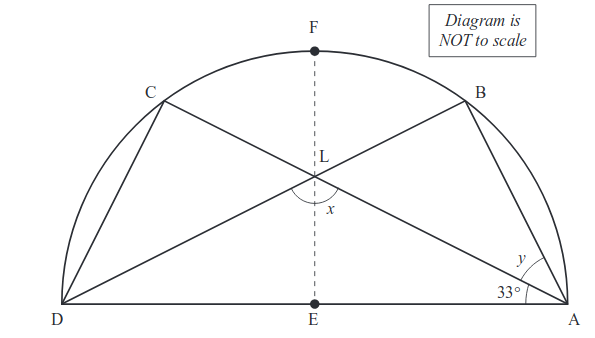
\includegraphics[width=0.6\textwidth]{semicircle}
            \end{center}
            The diameter of the semicircle is $ AD $. The construction is symmetric about the line $ EF $. Calculate the
            values of $ x $ and $ y $.
  \question Consider two lines. One passes through the points $ (0,3) $ and $ (2,5) $; the other passes through the points $ (3,4) $ and $ (5, 6) $.
            Either find the point of intersection, or use precise mathematical reasoning to show that they do not intersect.
\end{questions}

\end{document}
